%%%%%%%%%%%%%%%%%%%%%%%%%%%%%%%%%%%%%%%%%%%%%%%%%%%%%%%%%%%%%%%%%%%%%%%%%%%%%%%%
% Author : [Name] [Surname], Tomas Polasek (template)
% Description : Seventh exercise in the Introduction to Game Development course.
%   It deals with the creation of a Game Design Document, presenting a short 
%   pitch for a potential game project.
%%%%%%%%%%%%%%%%%%%%%%%%%%%%%%%%%%%%%%%%%%%%%%%%%%%%%%%%%%%%%%%%%%%%%%%%%%%%%%%%

\documentclass[a4paper,10pt,english]{article}

\usepackage[left=2.50cm,right=2.50cm,top=1.50cm,bottom=2.50cm]{geometry}
\usepackage[utf8]{inputenc}

% Hyper-Text References
\usepackage{hyperref}
\hypersetup{colorlinks=true, urlcolor=blue}

% Drawing Images and Graphs
\usepackage{tikz}
\usepackage{pgfplots}

% Page Utilities
\usepackage{graphicx}

% Image Sub-Captions
\usepackage{subcaption}

\newcommand{\ph}[1]{\textit{[#1]}}

\title{%
Game Pitch Document%
}
\author{%
[Name] [Surname] ([Login])%
}
\date{}

\begin{document}

\maketitle
\thispagestyle{empty}

{%
\large

\begin{itemize}

\item[] \textbf{Title:} \ph{Working Name or Title}

\item[] \textbf{Genre:} \ph{Full Genre}

\item[] \textbf{Style:} \ph{2D/3D, Style, Visual}

\item[] \textbf{Platform:} \ph{Initial and Potential Platforms}

\item[] \textbf{Market:} \ph{Target Market / Demographic}

\item[] \textbf{Elevator Pitch:} \ph{``One-Liner'' Pitch (10-30 words max)}

\end{itemize}

}

\section*{\centering The Pitch}

\ph{Replace all text in this section with the game design pitch...}

\subsection*{Instructions}

In this exercise, you assume the role of an enterprising game developer who has a great idea for a new game -- \emph{The Game}. You are tasked with the creation of a short \emph{Game Design Document}. That is, a \emph{pitch} of The Game's main idea to potential \emph{investors} or \emph{leadership} of a game studio. If you have your own ideas for a game, this is a great opportunity to develop them further. Alternatively, you can also choose an already existing game, but I recommend trying to come up with your own idea first. 

Within this template, you will find placeholders and hints \ph{like this one}, which you should read and replace with your own text. You can use any means of expression you deem appropriate -- text, reference images from other games, sketches, diagrams, tables, graphs, etc. Remember the goal: ``selling'' your idea so that you get the opportunity to actually \emph{make} The Game. Keep it brief and to the point. The length of your final document \textbf{shouldn't exceed 2-3 pages}. Following are example sections and pointers as to what they could contain. However, the document structure is certainly not set in stone. Feel free to modify it as necessary.

\subsection*{Introduction}
This should be the core of your pitch. Describe what \emph{exactly} it is you want to make. What is \emph{important}, what makes your game \emph{special}. All in one paragraph (50 words max).

\subsection*{Background}
What lead you to The Game's basic idea? What are the inspirations -- other games (even physical), sports, events, etc. Is it a continuation of some long-going traditional genre? Are you trying to bring back something that worked in the past?

\subsection*{Setting}
Describe the setting of your game. Is your game \emph{narrative-based}? You should detail the basic plot here. Cover the character of your \emph{protagonist} and their interaction with the environment. Will your story be \emph{interactive}? You can put some example dialogues and possible choices here as well. Even games with \emph{light} or \emph{no narrative} take place in some kind of universe.

\subsection*{Features}
What are the main \emph{selling points} of your game? Think about the \emph{target market} and \emph{market values} of your game. What makes it unique among other, already existing games? Why would players want to play \emph{your} game instead of some other? You can use a bullet point list or combine it with a \emph{value graph}.

\begin{figure}[h]

\centering
    
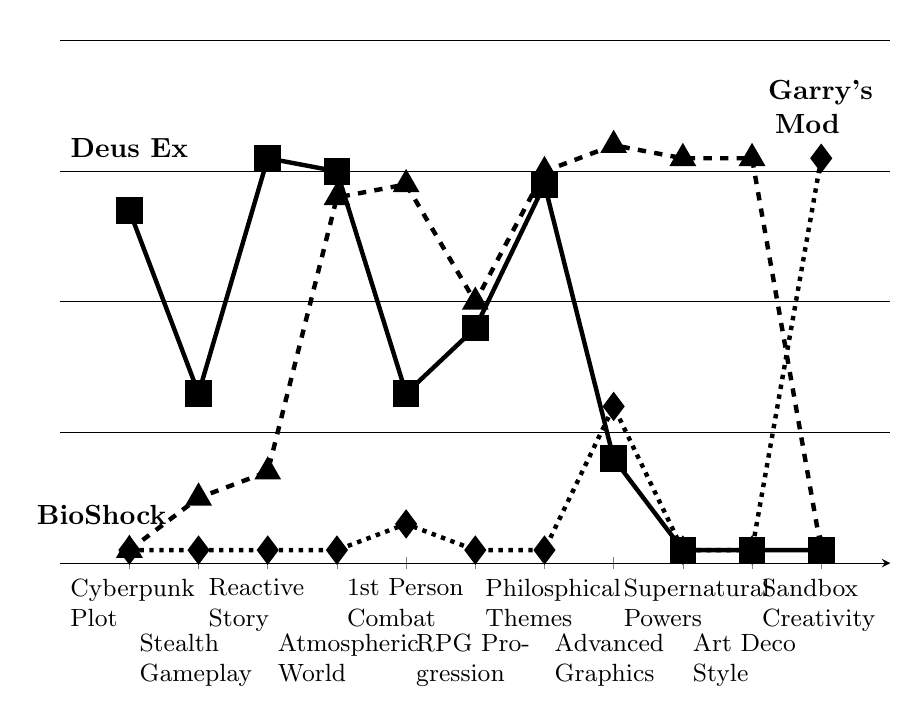
\begin{tikzpicture}[remember picture]%
\begin{axis}[
    domain=0:1, 
    clip=false, 
    ymin=0, xmin=0, ymax=4.1, xmax=12, 
    xtick={1,2,...,11}, 
    yticklabels={}, 
    xticklabels={Cyberpunk Plot, Stealth Gameplay, Reactive Story, Atmospheric World, 1st Person Combat, RPG Progression, Philosphical Themes, Advanced Graphics, Supernatural Powers, Art Deco Style, Sandbox Creativity}, 
    xticklabel style={yshift={-mod(\ticknum, 2) * 2em}, text width=1.5cm, font=\small}, 
    y tick style={draw=none}, 
    x axis line style={|-|}, 
    y axis line style={draw=none}, 
    axis lines=middle, 
    width=\linewidth, 
    height=0.3\paperheight
]
    \addplot [ultra thick, mark=square*, mark options={scale=2,solid}] coordinates {
        (1, 2.7)
        (2, 1.3)
        (3, 3.1)
        (4, 3.0)
        (5, 1.3)
        (6, 1.8)
        (7, 2.9)
        (8, 0.8)
        (9, 0.1)
        (10, 0.1)
        (11, 0.1)
    } node[above, yshift=15pt, pos=0] {\textbf{Deus Ex}};
    
    \addplot [ultra thick, dashed, mark=triangle*, mark options={scale=2,solid}] coordinates {
        (1, 0.1)
        (2, 0.5)
        (3, 0.7)
        (4, 2.8)
        (5, 2.9)
        (6, 2.0)
        (7, 3.0)
        (8, 3.2)
        (9, 3.1)
        (10, 3.1)
        (11, 0.1)
    } node[above, yshift=5pt, xshift=-10pt, pos=0] {\textbf{BioShock}};
    
    \addplot [ultra thick, dotted, mark=diamond*, mark options={scale=2,solid}] coordinates {
        (1, 0.1)
        (2, 0.1)
        (3, 0.1)
        (4, 0.1)
        (5, 0.3)
        (6, 0.1)
        (7, 0.1)
        (8, 1.2)
        (9, 0.1)
        (10, 0.1)
        (11, 3.1)
    } node[above, yshift=5pt, xshift=-5pt, pos=1, text width=1cm, align=center] {\textbf{Garry's Mod}};
    
	\draw [] (axis cs:{0,1}) -- (axis cs:{12,1});
	\draw [] (axis cs:{0,2}) -- (axis cs:{12,2});
	\draw [] (axis cs:{0,3}) -- (axis cs:{12,3});
	\draw [] (axis cs:{0,4}) -- (axis cs:{12,4});
\end{axis}
\end{tikzpicture}

\caption{Example value graph for \emph{Deus Ex}, \emph{BioShock}, and \emph{Garry's Mod}.}
\label{Fig:ValueGraph}

\end{figure}

\subsection*{Genre}
Specify the genre of The Game. Be \emph{clear}, but be sure to note on the \emph{nuances} which set your game apart from others within the same genre. 

\subsection*{Platform}
What are the platforms you plan to release The Game on? Do you have a core set in mind? Are you going to release versions for other platforms later?

\subsection*{Style}
Here, you can provide a visualization of what The Game would look like. Don't have concept artist at hand? Use diagrams, schemes, or illustrate on images from already existing games. It is time to dust off your \emph{Microsoft Paint} skills!

\begin{figure}[h]

\centering

\begin{subfigure}{0.29\linewidth}
\includegraphics[width=\linewidth]{example-image-a}
\captionof{figure}{Style Exhibit 1a.}
\label{Fig:Style1A}
\end{subfigure}\hfill
%
\begin{subfigure}{0.29\linewidth}
\includegraphics[width=\linewidth]{example-image-b}
\captionof{figure}{Style Exhibit 1b.}
\label{Fig:Style1B}
\end{subfigure}\hfill
%
\begin{subfigure}{0.29\linewidth}
\includegraphics[width=\linewidth]{example-image-c}
\captionof{figure}{Style Exhibit 1c.}
\label{Fig:Style1C}
\end{subfigure}

\end{figure}

\subsection*{Formatting \& Submission}

Your submission should follow a similar \textbf{structure} to this template. You can either use the provided \LaTeX\ template or roughly replicate it in some other text processing software. The format of the section ``\emph{The Pitch}'' is left up to you. For inspiration, see the game design documents included on the \href{http://cphoto.fit.vutbr.cz/ludo/courses/izhv/exercises/e7/}{assignment page}, or the lecture dedicated to \href{http://cphoto.fit.vutbr.cz/ludo/courses/izhv/lectures/l12/}{game development}. The only accepted document format is \textbf{pdf}. You can submit the pdf by following the submission guidelines detailed on the \href{http://cphoto.fit.vutbr.cz/ludo/courses/izhv/exercises/sub/}{course's website}. 

\end{document}
